\chapter{Background}

In this chapter we introduce the basic concepts that are the focus of this thesis, such as \wsns and \textit{Data Minimization}. It should provide an explanation to the technologies and issues that serve as the motivation for the thesis. % we still start by giving some areas to the research into DM and reasons for it.

%\textit{This section should cover some background information to give the reader some background knowledge to what the project has been about that is required knowledge before moving forward.}

\section{Wireless Sensor Network (WSN)}

%describe my idea of a sensor network and how I will look at them for the sake of the thesis. (node/server/environment)

% how it's built up (components)

\wsns are a growing interest in the research community \cite{wsnsurvey, akyildiz2007survey, min2001low}. The attention drawn to them can be motivated by new applications that are enabled from these large-scale networks of small devices that can collect information from a physical environment.

A \wsn is an improvement from the traditional sensor networks, made possible by advances in micro-electro-mechanical systems (MEMS) technology\cite{sohrabi2000protocols, min2001low} making sensor nodes that are smaller, multifunction and cheaper in comparison to previous sensors. 

\begin{figure}[ht]
    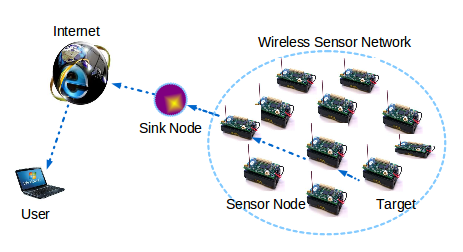
\includegraphics{include/figures/WSN_illu}
    \caption{An illustration of a \wsn}
    \label{fig:wsn_illustration}
\end{figure}

Traditional sensors have two ways of being deployed; 1) They were positioned far away from the actual \textit{phenomenon} (e.g. something known by sense perception) which required large sensors using complex techniques to distinguish the targets from surrounding noise. 2) Several sensors were deployed that only performed sensing and their communication topology had to be carefully engineered and they transmitted time series of the data to the central nodes which performed the communication.\wsns on the other hand, is constructed by deploying a large number of sensor nodes close to the phenomenon and their position doesn't need to be engineered or predetermined\cite{wsnsurvey}. 

% add some examples of practical WSN applications % add from wsnsurvey? % http://www.chicagotribune.com/bluesky/originals/ct-array-of-things-privacy-policy-bsi-20160610-story.html - wsn example

Sensor networks can be built up by many different types of sensors such as acoustic, seismic, infrared, thermal, radar or visual, which can monitor an assortment of environmental conditions\cite{estrin1999next}, e.g. temperature, humidity, pressure, noise levels. 

These features that \wsns supports, makes them available for a wide range of usages. For example, the city of Chicago began a project\cite{chicago2016} to install \wsn for tracking information on urban conditions. The sensors are planned to be low-resolution cameras, infrared cameras and microphones for analyzing urban areas and sending the information back to a secure remote server. The article stresses that even though the sensors would have a low-resolution cameras, the video could still be used to identify individuals. Which could cause a privacy concern. To prevent this, that project will also define a privacy policy before installing the sensors, through public hearings and also informing the public what kind of information and how the information would be gathered.

There are many other practical applications for \wsns some examples include environmental applications; for tracking small animals and birds, monitoring air pollution and precision agriculture\cite{baggio2005wireless,collier2010acoustic, khedo2010wireless}. In military applications for mission and flight systems in situ sensing and self-adapting mine-fields\cite{vardhan2000wireless, merrill2003collaborative}. Also in health-care applications for drug administration and large-scale monitoring of stress in the field\cite{darwish2011wearable, ertin2011autosense}.

% Other examples of 

% privacy policy

% https://pdfs.semanticscholar.org/2644/b8c7f4e488f3ce4c56382c4affda2e5e98fa.pdf

%% does this need more information? it's just a network of sensor nodes?

%\section{Privacy} The justification and importance of privacy is done in different ways. For example, Bloustein claims privacy as a neccessity for human dignity\cite{bloustein1964privacy}. Gavison 

\section{Privacy Issues in WSNs}

% TB Added

% other privacy issues than DM

When adversaries can access to sensitive information in \wsn, it's a privacy issue. This can either be achieved by accessing sensor data or eavesdropping on communications in the network. For example, if an adversary gains access to data from sensors monitoring a home on both the inside and the outside, they could derive information regarding the inhabitants' behaviours or private activities. 

% In order to prevent this, different security protocols are used. But previously proposed security mechanisms but due to the inherent properties of sensor networks these protocols are rendered impractical. 

% security in wsns 

Furthermore, there are many other issues related to privacy. In a paper by Haowen and Perrig\cite{chan2003security}, they state that the main problem related to privacy is that the information from sensor nodes are aggrevated and can be accessed remotely. This makes it easier for adversaries to access information in a low-risk and anonymous manner. Also making it possible for just one adversary to monitor multiple sites at once. 

% https://pdfs.semanticscholar.org/2644/b8c7f4e488f3ce4c56382c4affda2e5e98fa.pdf

%In another paper, by Slijepcevic, Wong and Potkonjak, list four major challenges\ref{slijepcevic2004security} in regards to \wsn. Firstly \textit{hostile environment}, regarding \wsns deployed by the military upon battlefields. In those cases the nodes can't be protected from physical attacks. 

Finally, a major issue was mentioned in an paper by Al Ameen, Liu and Kwak\cite{al2012security}, as privacy is a major concern in healthcare applications. They claimed that if the privacy issues aren't honestly debated, there is a risk for public backlash that will result in mistrust and might make available technology not used. This can happen either if the data is obtained with or without the consent of the person, since the damage can happen either way.



%Another issue regarding \wsn privacy was mentioned in a paper by Slijepcevic, Wong and Potkonjak\ref{slijepcevic2004security}. Applications strives to collect as much data with a precision of the sensing data as possible, except in some special cases, to have the best performance possible. Although this is in duality to privacy protection, which strives for the minimum amount of data for a single individual. 

% http://link.springer.com/article/10.1007/s10916-010-9449-4

% discuss misuse / disbelief and ppl not using the system

\section{Data Minimization}

% discuss DM from an abstract POV. Social > Legal > Technical, since there isn't much technical articles regarding DM & WSNs. 

As defined by the EDPS (European Data Protection Supervisor); "The principle of data minimization means that a data controller should limit the collection of personal information to what is directly relevant and necessary to accomplish a specified purpose."\cite{websiteEu} %discuss privacy?

%They should also retain the data only for as long as is necessary to fulfil that purpose.

%This makes it an important aspect of privacy in data-collecting settings. 

With the world becoming more and more digitalized, the collection of personal data from users becomes a growing concern. Today, data processing entities automatically makes decisions based on data analysis which can impact the lives of individuals, which in turn makes the need for protecting their personal data is even greater.\cite{danezis2015privacy} Another problem which arises from being more connected is that individuals, whose data is being collected, are often unaware of the consequences of the data processing that comes after. Also, legal repercussions for infringement of data protection obligations is usually only due to a breach or a misuse that has already occured. There are systems that support this thinking, that requires users to know what data is being collected, such as Privacy Enchaning Information Management Systems (PE-IMS) which will be discussed later on in this chapter. \\

% to have privacy is a fundamental right for everyone. 

% from this discussion extract what DM seeks to prevent?

% maybe this is a too general paragraph that is too short, should be converted to a more arguing paragraph leading up to the more precise definitions.

In a paper by Pfitzmann, Andreas and Hansen and Marit, a combined terminology for the aspects of Data Minimization was defined. The main definitions they used were: \textit{Anonymity}, \textit{Unlinkability}, \textit{Undetectability} and \textit{Unobservability}\cite{pfitzmann2010z}. These definitions sought to explain data minimization. To explain these definitions, we will use the same terminology as in the paper, where the two most important ones are \textit{subjects} and \textit{Items of Interest} (IOI). 

For privacy reasons, being that we wish to maximize it for human beings, subjects are mainly users in a system. But in the definitions that follow, it can be a legal person or even be a computer. An Item of Interest is a generalization of what can be seen as information, e.g. the contents of a message, the name or the pseudonym of a user or even the action of a user sending a message. All of these can be an Item of Interest, and the definitions are stated in the following list: \\

% persons communicating in the system are \textit{subjects} and the information is regarded as \textit{Items of interest} (IOI). % is this obvious? Should IOIs be better defined?

% It should be noted that this reference isn't as carefully finished as other papers. It seems to be a work in progress and it should perhaps be mentioned in the text.

%It should be noted that the definitions are written with regards to an attacker's perspective. 

\begin{itemize}
\setlength\itemsep{1em}
\item[] \textbf{Anonymity} means that for a subject to have anonymity, it has to be indistinguisable in a set of subjects. Meaning that if a subject has a set of attributes defining the subject, there always has to exist an appropriate set of subjects with potentially the same attributes, in other words: "Anonymity of a subject means that the subject is not identifiable within a set of subjects, the \textit{anonymity set}.", where the anonymity set is the set of all possible subjects. The opposite of anonymity is called \textit{Identifiability}. 

\item[] \textbf{Unlinkability} is the relation between IOIs in the system. If several IOIs become compromised, an attacker should not be able to distinguish whether these IOIs are related or not. The opposite of unlinkability is called \textit{Linkability}.

\item[] \textbf{Undetectability} is an attribute for an IOI. It means that an attacker should not be able to distinguish whether the item exists or not. The opposite of undetectability is called \textit{Detectability}.

\item[] \textbf{Unobservability} is an attribute which is combination of \textit{anonymity} and \textit{undetectability}. It means that, in regards to an IOI, that neither if a subject is involved in the IOI or not, he or she should be aware of the other involved subjects. The opposite of unobservability is called \textit{Observability}.
\end{itemize}

% discuss these definitions in a setting? todo on this from prev paragraph

%TBR: This covers two important aspects of data minimization, the first being that data should only be kept for as long as it is useful for an application and the second being that they should only collect "relevant" data. The latter is more interesting to the project, since the project's aim is to solve part of this problem. %why is this a good a good definition for me?

\subsection{Over-Collection}

In contrast to Data Minimization, there is a term called Data Over-Collection. In a paper by Yibin Li et al\ref{li2016privacy}, they adressed issues of data over-collection and presented a privacy protection framework to solve them. Their focus was the "smart city", an urban development vision with social facilities being connected wirelessly with information and communication technology and IoT-technology in a secure fashion to improve the efficiency of services. The system would help identify users in a smart fashion to relieve the need of ID- or credit cards. This requires that smart cities have a system that contains a lot of different users' information, which puts the users at a potential privacy leakage when accessing these features. They also sought to prevent over-collection of data, but though a privacy protection. Their definition of data over-collection was; "Collecting data more than enough on it's original function while within the permission scope". This definition is related to that their target, for which they sought to minimize over-collection, was smartphones. An example they used for explaining this definition was the following: "I take a picture and want to share it with my friends via some SNS app in my smartphone. For sharing this photo to my friends, I have to agree the permission request from this app. After authorize the access permission to this SNS app, all my photos are available to this app, but I only want this app to access one specific photo. As a result, this app may collect data more than enough on my original requirement while within the permission scope which I authorize." 


\section{Modelling Concurrency}

In this section we will present some different approaches to modelling concurrency. These will give an insight into the other tools available, the chosen approach for this thesis (Model Checking) will not be described here but will be thoroughly explained in the next chapter.

\subsection{Petri Nets}

In 1962, Carl Adam Petri disserted his work on a more graphical way of modelling concurrency, namely using something called \textit{Petri Nets}. A Petri Net is a directed bipartite graph. An example can be seen in Figure~\ref{fig:petri_net}. Each node in the graph represent transitions, shown as bars, or places, which are shown as circles. The black dots at places are called tokens, they indicate the holding of a condition at that place. Connecting the nodes are directed arcs that describe pre- and/or postconditions for the transitions, illustrated as arrows. 
% discuss input and output?
% discuss tokens?
% mention arc-weights?

% https://upload.wikimedia.org/wikipedia/commons/f/fe/Detailed_petri_net.png
\begin{figure}[h]
    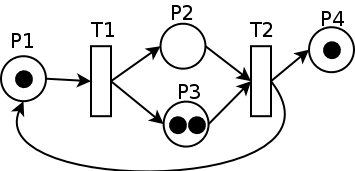
\includegraphics[scale=0.5]{include/figures/petri_net}
    \caption{Illustration of a Petri Net}
    \label{fig:petri_net}
\end{figure}

The primary rule for Petri Net theory is the rule for transition enabling and firing. It derives from the idea that many systems can be described as system states and their changes. So to simulate the behavior of a system, each state or marking are allowed to change according to the following rule:\\

\begin{itemize}
	\setlength\itemsep{1em}
	\item A transition is enabled iff each of its input places has atleast one token
	\item A transition can only fire if it is enabled.
	\item When a transition fires it removes a token from each of its input places and a token is deposited into each of its output places.\\
\end{itemize}

%\begin{itemize} alt. description
%\item A transition t is said to be enabled if each input p of t is marked with at least w (p,t) tokens, where w(p,t) is the weight of the arc from p to t. 
%\item An enabled transition may or may not fire (depending on whether or not the event takes place).
%\item A firing of an enabled transition t removes w(p,t) tokens from each input place p of t, and adds w(t,p) tokens to each ouput place p of t, where w(t,p) is the weight of the arc from t to p.
%\end{itemize} 

By analyzing different properties of a Petri net model of a system, such as liveness and boundedness, one can prove other properties aswell. For example, a Petri net is said to be \textit{live}, if there always exist a fire sequence to each transition in the model, and if the model is live it's also guaranteed to be free of deadlock\cite{ramamoorthy1980performance}. A Petri net is said to be \textit{k-bounded} if for each place, there exists an upper bound \textit{k}, for how many tokens that can be there simultaneously. If \textit{k} is 1, then the system is said to be \textit{safe}. % mention initial marking?

% give perhaps some disadvantage to this application, not required.

% discuss further developments such as Colored Petri Nets?

\subsection{Process Calculi}

\textit{Process Calculi} is a family of related approaches for formal modelling of concurrent systems. It allows for a high-level description of the interaction, communication and the synchronization between processes and agents. %wikiwiki
Some examples of different Process Calculi are CSP, LOTOS and $\pi$-calculus\cite{baeten2005brief}. Their focus vary, for they are specialized on modelling different systems, but some features they (and other Process Calculi) share are: \\

\begin{itemize}
	\setlength\itemsep{1em}

\item Interaction between processes are represented as communication(message-passing), rather than manipulation of shared variables. %interactions 
\item Processes are described as a collection of primitives and operators for those primitives. %processes
\item Algebraic laws are defined for the process operators, which allows them to be analyzed by \textit{equational reasoning}. \\ %algebraic laws
\end{itemize}

Initially, to define a \textit{process calculus}, you start with a set of channels as a means of communication. The internal structure of channels are rich and are constructed to improve efficiency, but when explained theoretically these improvements are usually abstracted away. Also, a way to form new processes from old ones is required, this also varies from the different implementations but what they have in common can be summarized the following: \\ %durr?

\begin{itemize}
	\setlength\itemsep{1em}
\item A way of expressing parallell composition of processes
\item A way of specifying which channels are used for sending and receiving data
\item A way to sequentialize interactions
\item A way to hide interaction points
\item Recursion or a way to process replication \\
\end{itemize}

% show an example of a language described in PC
Furthermore, an example of constructing a process calculus model can be seen in the CRC Handbook of Computer Science and Engineering\cite{pierce1997foundational}, written in $\pi$-calculus and compared to $\lambda$-calculus. % mention it's not relevant to present?

\section{Related Work}

This section will present some related work into also ensuring privacy for users, where other approaches than the one in this thesis were used.

\subsection{Data Erasure and Declassification}

% it's different, but try explain the duality of it and DM. mention outside scope

% some background

Another step to consider when ensuring privacy for users having their data collected is the aspect of releasing or removing the data. In many systems, both of these functionalities are required. For this sake, different policies for \textit{erasure} and \textit{declassification} need to be clearly specified so the users' privacy is protected. 

% how it's used (maybe list one or two examples)

In an paper by Chong and Myers\cite{chong2005language}, they propose a security policy framework where policies for both can be specified so it suits the desired application. In said framework, one would specify an erasure policy on under which conditions information must be erased. One could also state what policy that would allow data to survive erasure, since information could be allowed to still exist within a system in a restricted form. Secondly, declassification policies would define what policy should be enforced on new information, the conditions under which said information would be declassified and finally the policy it should have after declassification. 

% Declassifying information means that information that is classified as secret ceases to be to restricted. 

This approach covers an important aspect of privacy, namely the managing of personal data. This differs from the focus of the thesis, as we seek to minimize the collection of data to achieve better privacy. % say something more about the difference/similarities 

% how it differs from DM
%This approach to ensuring privacy on personal data is closely related to data minimization, as it covers another aspect of data minimization namely the storing on personal data as long as it's required. 

\subsection{Privacy Enhancing Identity Management Systems (PE-IMS)}

% use definitions in previous section in this section aswell for explanations, this is already done in the article/paper/smth?

In an online setting, it's assumed that people would like to retain their anononymity.\cite{hansen2004privacy} To let users manually control their identities would be a cumbersome process, so instead an automated solution managing this would be preferred. Such a solution can be an Identity Management System (IMS).

An IMS is a system that allows support for "administration of information subjects". An extension of this is Privacy-Enhancing Identity Management Systems (PE-IMS) which supports "active management of personal information" which grants all parties involved flexibility and control over their personal data. A principle used for this is called 'Notice and Choice', a central aspect of data minimization, which means user-controlled linkability of personal data. This puts the responsibility on the user to make informed choices of representing and managing their partial identities.

This allows a user to be as anonymous as they wish, within the predefined limits, since a PE-IMS can be designed to offer any degree of anonymity and linkability. Applications utilizing PE-IMS would specify the range of choices available to the user. Some applications might require some authenticity from the user, e.g. government processes, and in other cases a user could be allowed complete anonymity. By allowing each application different levels of authorization, one can minimize linkability between different communication events and still maximize information exchange while preventing context-spanning profiling. % this section has a lot from the paper.

% --- 
%\textit{compare this to your work}

%\subsection{Security and Privacy for Mobile Electronic Health Monitoring and Recording Systems}
%\todo{Health applications using DM}\cite{barnickel2010security}
%\textit{discuss how healthnet works}
%In a paper from 2010 Barnickel, Karahan and Meyer investigated a mobile health monitoring and data collection system called HealthNet, which is a joint research project of several research groups of RWTH Aachen University. The system consists of a sensor network embedded in a users clothing which collects vital parameters and wirelessly communicates it to the wearer's phone. From there the data is managed, stored and transfered securely to relevant parties, such as medical experts, emergency care and private parties trusted by the wearer. By using the phone the user can control who may access the data. The system is deisgned so that the emergency support can be managed automatically when the vital signs match predefined patterns and not to create an infrastructure among medical experts or health insurance companies. Confidentially and integrity is managed through cryptographic techniques, which prevent attacks on the transmissions and stolen devices. 
%\textit{find the entry point for discussing DM}

%\subsection{Smart City} 
%\label{section:SmartCity}

%\textit{some background into their approach}\cite{li2016privacy}
%\textit{some comparison to this project}
%*discuss smart city's approach in difference to your own*
% ---
